%%%%%%%%%%%%%%%%%%%%%%%%%%%%%%%%%%%%%%%%%
% Beamer Presentation
% LaTeX Template
% Version 1.0 (10/11/12)
%
% This template has been downloaded from:
% http://www.LaTeXTemplates.com
%
% License:
% CC BY-NC-SA 3.0 (http://creativecommons.org/licenses/by-nc-sa/3.0/)
%
%%%%%%%%%%%%%%%%%%%%%%%%%%%%%%%%%%%%%%%%%

%----------------------------------------------------------------------------------------
%	PACKAGES AND THEMES
%----------------------------------------------------------------------------------------

\documentclass{beamer}

\mode<presentation> {

% The Beamer class comes with a number of default slide themes
% which change the colors and layouts of slides. Below this is a list
% of all the themes, uncomment each in turn to see what they look like.

%\usetheme{default}
%\usetheme{AnnArbor}
%\usetheme{Antibes}
%\usetheme{Bergen}
%\usetheme{Berkeley}
%\usetheme{Berlin}
%\usetheme{Boadilla}
%\usetheme{CambridgeUS}
%\usetheme{Copenhagen}
%\usetheme{Darmstadt}
%\usetheme{Dresden}
%\usetheme{Frankfurt}
%\usetheme{Goettingen}
%\usetheme{Hannover}
%\usetheme{Ilmenau}
%\usetheme{JuanLesPins}
%\usetheme{Luebeck}
%\usetheme{Madrid}
%\usetheme{Malmoe}
%\usetheme{Marburg}
%\usetheme{Montpellier}
\usetheme{PaloAlto}
%\usetheme{Pittsburgh}
% \usetheme{Rochester}
%\usetheme{Singapore}
%\usetheme{Szeged}
%\usetheme{Warsaw}

% As well as themes, the Beamer class has a number of color themes
% for any slide theme. Uncomment each of these in turn to see how it
% changes the colors of your current slide theme.

%\usecolortheme{albatross}
%\usecolortheme{beaver}
%\usecolortheme{beetle}
%\usecolortheme{crane}
%\usecolortheme{dolphin}
%\usecolortheme{dove}
%\usecolortheme{fly}
%\usecolortheme{lily}
%\usecolortheme{orchid}
%\usecolortheme{rose}
%\usecolortheme{seagull}
%\usecolortheme{seahorse}
%\usecolortheme{whale}
%\usecolortheme{wolverine}

%\setbeamertemplate{footline} % To remove the footer line in all slides uncomment this line
%\setbeamertemplate{footline}[page number] % To replace the footer line in all slides with a simple slide count uncomment this line

%\setbeamertemplate{navigation symbols}{} % To remove the navigation symbols from the bottom of all slides uncomment this line
}

\usepackage{graphicx} % Allows including images
\usepackage{booktabs} % Allows the use of \toprule, \midrule and \bottomrule in tables


\usepackage[square, numbers, comma, sort&compress]{natbib} % Use the natbib reference package - read up on this to edit the reference style; if you want text (e.g. Smith et al., 2012) for the in-text references (instead of numbers), remove 'numbers' 
\usepackage{listings}
\usepackage{color}
\usepackage{xcolor}
\usepackage{textcomp}   %Iuse this for the degree symbol
\usepackage{amsmath}  % use for making bigger math symbols
\usepackage{relsize}  % use for making bigger math symbols

%----------------------------------------------------------------------------------------
%	TITLE PAGE
%----------------------------------------------------------------------------------------

\title[]{Mechanics Simulations With JavaScript} % The short title appears at the bottom of every slide, the full title is only on the title page

\author[]{Peter Krieg} % Your name
\institute[Bates College] % Your institution as it will appear on the bottom of every slide, may be shorthand to save space
{
Advisor: Gene Clough

\

Physics Fall Semester Thesis \\ % Your institution for the title page

\medskip
%\textit{john@smith.com} % Your email address
}

\date{\today} % Date, can be changed to a custom date

\begin{document}

\begin{frame}
\titlepage % Print the title page as the first slide
\end{frame}

%\begin{frame}
%\frametitle{Overview} % Table of contents slide, comment this block out to remove it
%\tableofcontents % Throughout your presentation, if you choose to use \section{} and \subsection{} commands, these will automatically be printed on this slide as an overview of your presentation
%\end{frame}

%----------------------------------------------------------------------------------------
%	PRESENTATION SLIDES
%----------------------------------------------------------------------------------------

%------------------------------------------------
\section{Overview} % Sections can be created in order to organize your presentation into discrete blocks, all sections and subsections are automatically printed in the table of contents as an overview of the talk
%------------------------------------------------


%\subsection{Subsection Example} % A subsection can be created just before a set of slides with a common theme to further break down your presentation into chunks
%
%\begin{frame}
%\frametitle{Paragraphs of Text}
%Sed iaculis dapibus gravida. Morbi sed tortor erat, nec interdum arcu. Sed id lorem lectus. Quisque viverra augue id sem ornare non aliquam nibh tristique. Aenean in ligula nisl. Nulla sed tellus ipsum. Donec vestibulum ligula non lorem vulputate fermentum accumsan neque mollis.\\~\\
%
%Sed diam enim, sagittis nec condimentum sit amet, ullamcorper sit amet libero. Aliquam vel dui orci, a porta odio. Nullam id suscipit ipsum. Aenean lobortis commodo sem, ut commodo leo gravida vitae. Pellentesque vehicula ante iaculis arcu pretium rutrum eget sit amet purus. Integer ornare nulla quis neque ultrices lobortis. Vestibulum ultrices tincidunt libero, quis commodo erat ullamcorper id.
%\end{frame}
%
%%------------------------------------------------

\begin{frame}
\frametitle{Overview - Why Did I Choose This Topic?}
\begin{itemize}
\item Use programming as a lens to view physics
\item Examine mechanics in more detail
\item Solve physics problems through simulations
\item JavaScript high level language -  viewable easily in web browser

\end{itemize}
\end{frame}

%------------------------------------------------


\begin{frame}
\frametitle{What is a simulation?}

\begin{itemize}

\item Animation vs. Simulation
\item Frames per second
\item File size

\vspace{1cm}
\begin{figure}[h] 
	\centering
		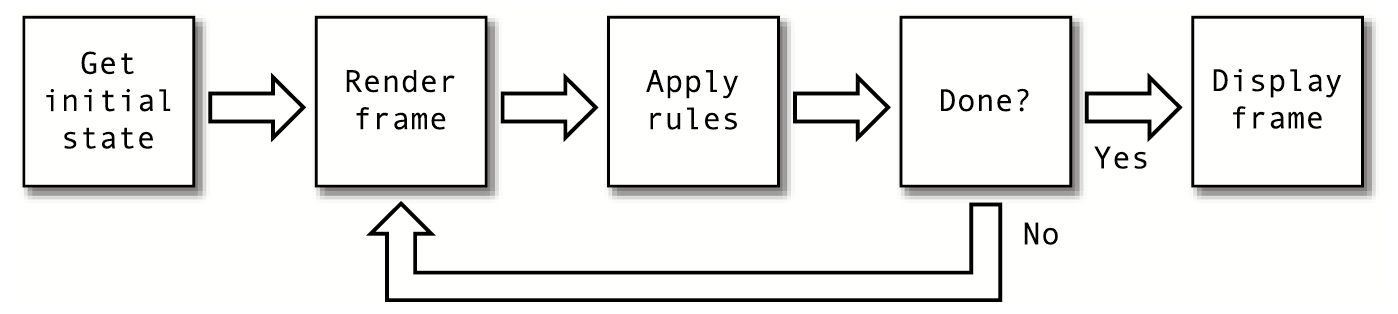
\includegraphics[width=8cm]{frames.png}

	\label{fig:frames}
\end{figure}
\end{itemize}
\end{frame}






\begin{frame}
\frametitle{Method of Basic Simulation}
\begin{itemize}

\item HTML5 canvas application programming interface (API)
\item Timer for each frame

\vspace{1cm}
\begin{figure}[h] 
	\centering
		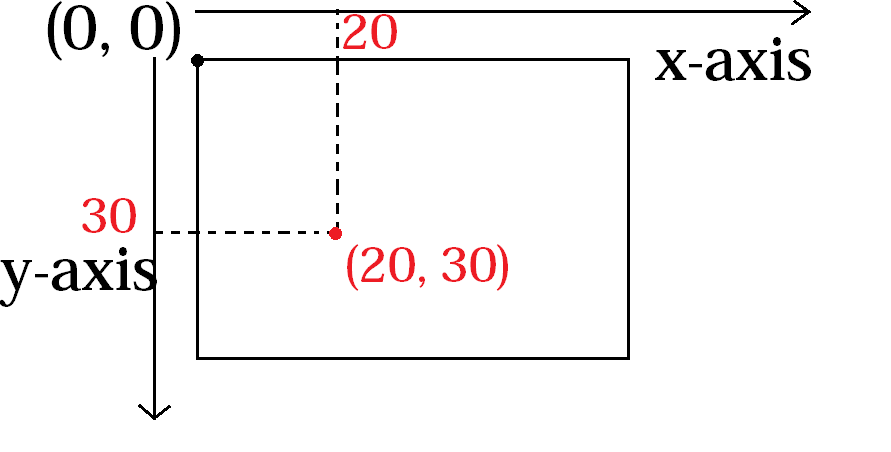
\includegraphics[width=7cm]{canvas.png}

	\label{fig:frames}
\end{figure}

\end{itemize}
\end{frame}





\section{Chapter 1}



\begin{frame}
\frametitle{Chapter 1: Basic Kinematics and Aerodynamic Drag}

\begin{itemize}
\item Three simulations
\item Simulation \#1: Basic bouncing ball
\item Simulation \#2: Bouncing ball with aerodynamic drag
\item Simulation \#3: Multiple bouncing balls

\end{itemize}
\end{frame}









\subsection{Simulation \#1}
\begin{frame}
\frametitle{Simulation \#1: Basic Bouncing Ball}

\begin{itemize}

\item Realistic g value

\item $
9.81 \hspace{1mm}  \frac{px}{s^2}  = .1635 \hspace{1mm}  \frac{\frac{px}{s}}{frame} \hspace{1mm}  \times \hspace{1mm}  \hspace{1mm}  \frac{60 frame}{s}
$

\vspace{1cm}
\item Coefficient of restitution ($C_r$)

\item $
C_r = \sqrt{\frac{KE_f}{KE_i}} = \sqrt{\frac{\frac{1}{2} mv_f^2}{\frac{1}{2} mv_i^2}} = \frac{v_f}{v_i}
$

\item $
v_f = v_i * C_r
$


\end{itemize}



\end{frame}



\subsection{Simulation \#2}

\begin{frame}
\frametitle{Simulation \#2: Bouncing Ball With Aerodynamic Drag}

\begin{itemize}

\item $ 
f_{d} = -\frac{1}{2}C_d \rho A v^2
$

\vspace{1cm}
\item  $ f_d =   $ force of drag
\item $\rho = $ density of fluid
\item $v = $ speed of object relative to fluid
\item  $C_d = $ drag coefficient (affected by texture, shape, viscosity, lift, etc)  
\item $ A = $ cross-sectional area of object


\end{itemize}





\end{frame}




\subsection{Simulation \#3}

\begin{frame}
\frametitle{Simulation \#3: Multiple Balls Bouncing}

\begin{itemize}

\item Same physics as simulation \#1
\item Array of ball objects
\item Each object has properties
\item Each frame cycles through array, updating properties of each object


\end{itemize}

\end{frame}


\section{Chapter 2}


\begin{frame}
\frametitle{Chapter 2: Planetary Motion}
\begin{itemize}
\item 3 Simulations
\item Simulation \#4: Orbits
\item Simulation \#5: Escape velocity
\item Simulation \#6: Kepler's 2nd law

\end{itemize}
\end{frame}

\subsection{Simulation \#4}

\begin{frame}
\frametitle{Simulation \#4: Orbits}

\begin{itemize}

\item Newton's Law of universal gravitation
\item $ 
F_g = G \frac{m_1 m_2}{r^2}  $

\vspace{1cm}
\item  Euler's Method to update velocity 
\item $
x(t+dt) = x(t) + \frac{dx}{dt}\left(t\right) dt
$



\end{itemize}

\end{frame}

\subsection{Simulation \#5}



\begin{frame}
\frametitle{Simulation \#5: Escape Velocity}

\begin{itemize}

\item $K_i + U_{g_{i}} = K_f + U_{g_{f}}$

\item $\frac{1}{2}mv_{esc}^2 - \frac{GMm}{r} = 0 + 0  $

\item $
v_{esc} = \sqrt{\frac{2GM}{r}}
$

\item $
 v_{esc} = \sqrt{\frac{2*1 \frac{px^3}{s^2}*1000000}{410 px}} \approx 69.843 \frac{px}{s} 
$
\vspace{1cm}

\item Used bigger canvas, and plotted velocities during planet's travel

\end{itemize}

\end{frame}



\begin{frame}
\frametitle{Simulation \#5: Escape Velocity}

\begin{figure}[h] 
	\centering
		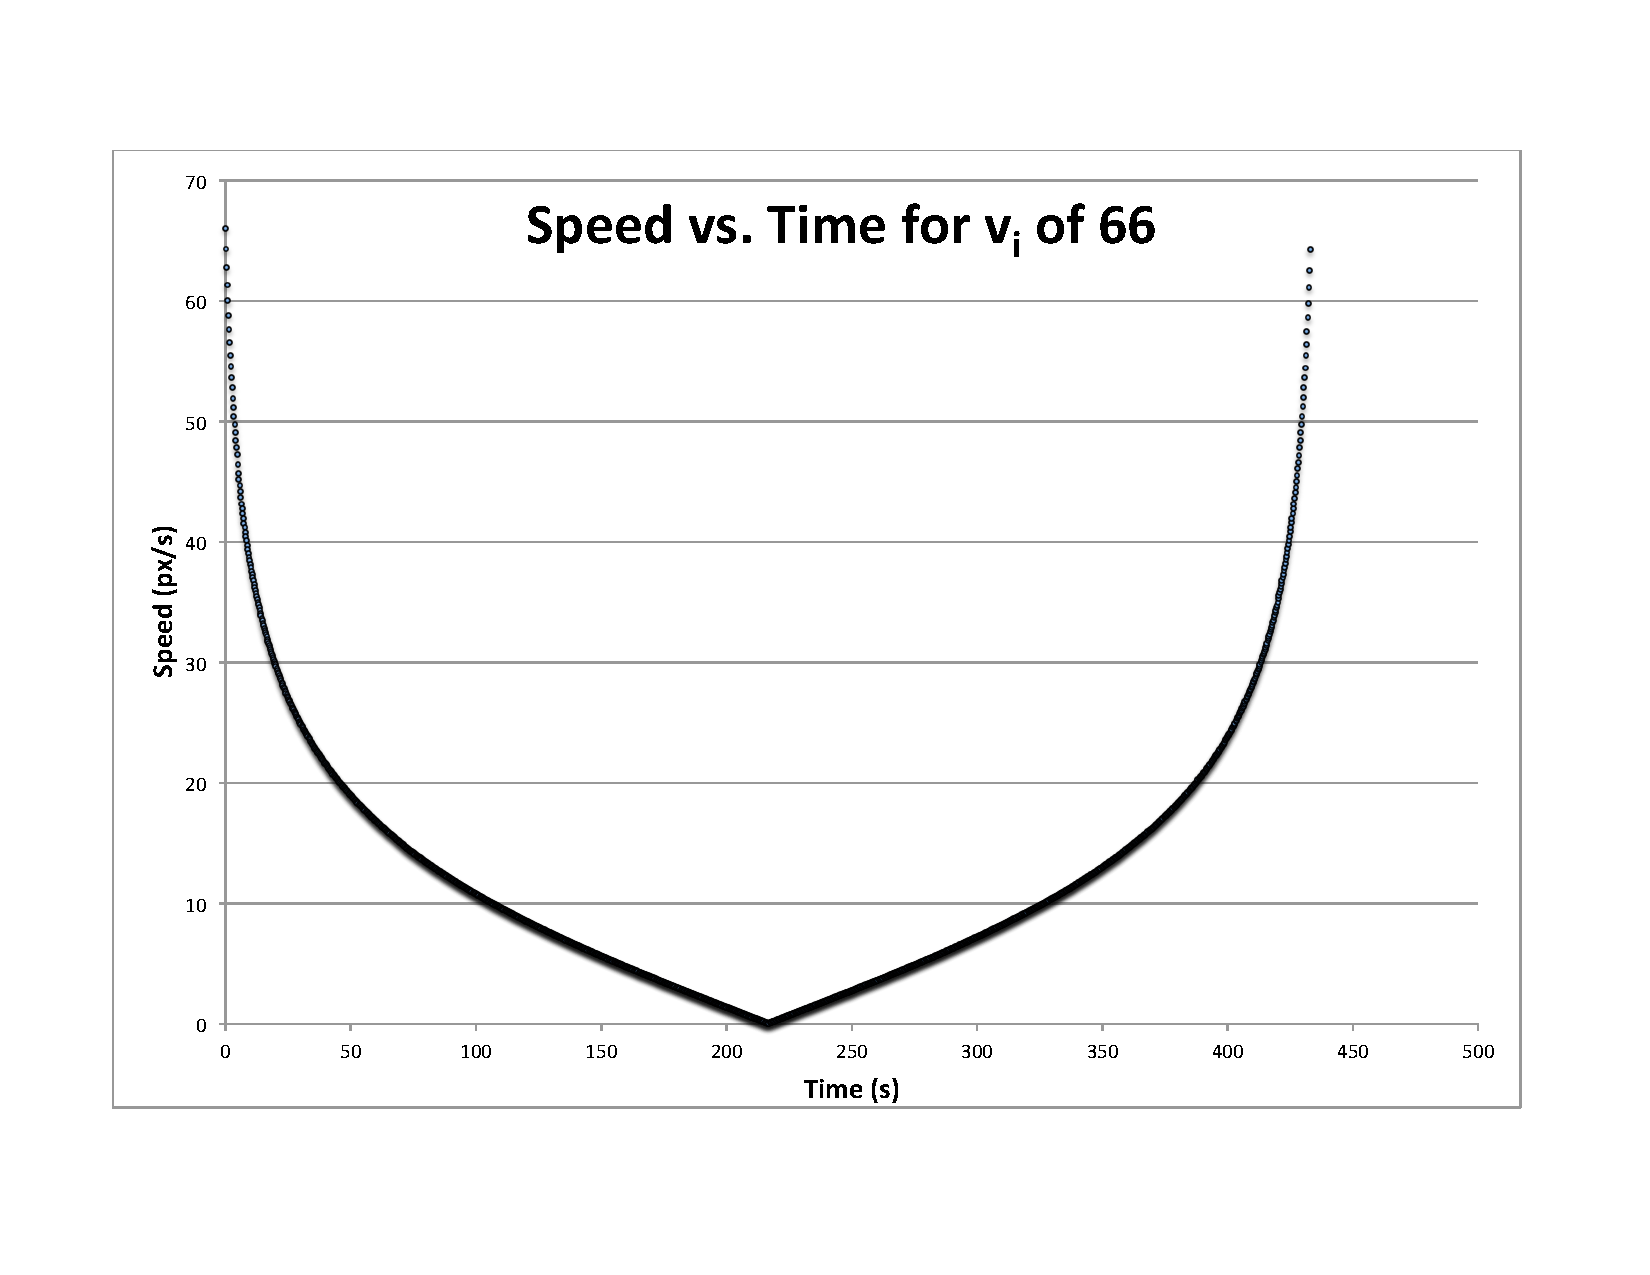
\includegraphics[width=9.5cm]{fig1.pdf}

	\label{fig:data1}
\end{figure}
\end{frame}


\begin{frame}
\frametitle{Simulation \#5: Escape Velocity}

\begin{figure}[h] 
	\centering
		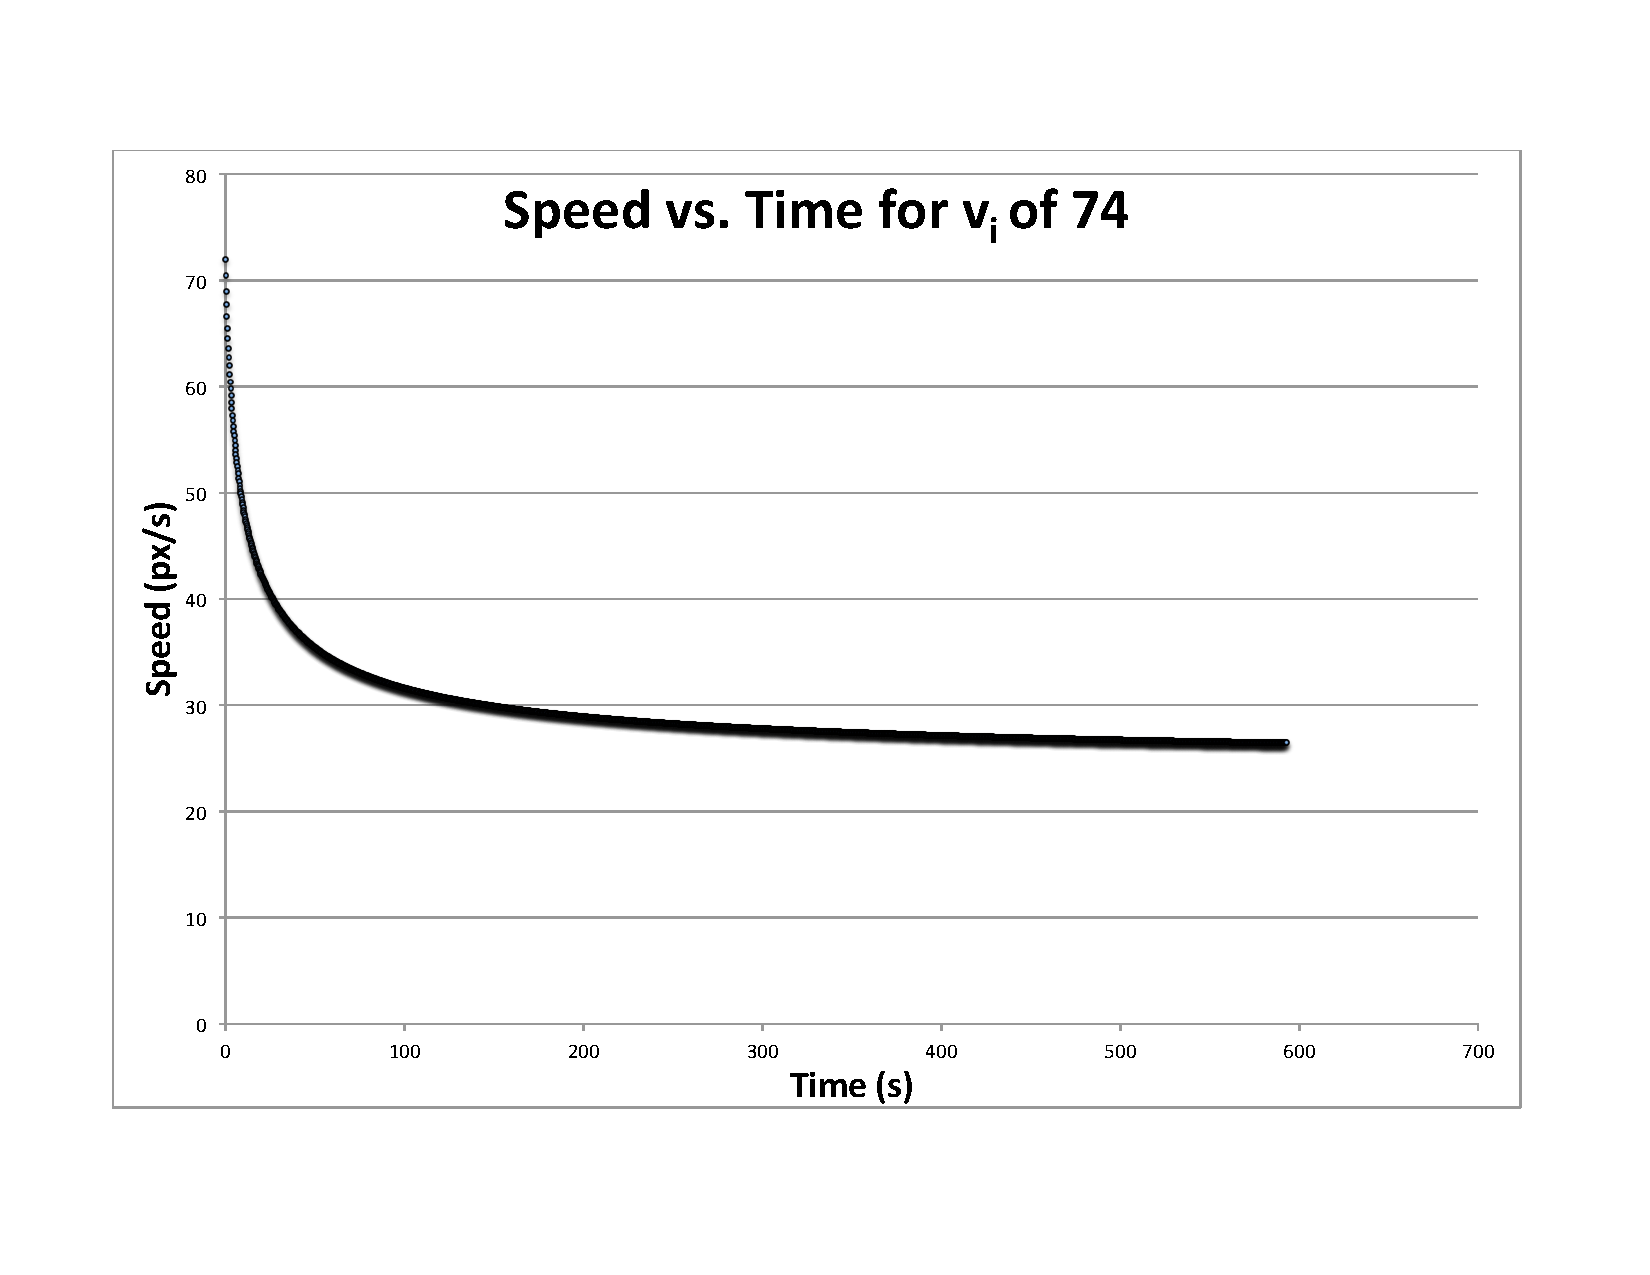
\includegraphics[width=9.5cm]{fig2.pdf}

	\label{fig:data1}
\end{figure}
\end{frame}

\begin{frame}
\frametitle{Simulation \#5: Escape Velocity}

\begin{figure}[h] 
	\centering
		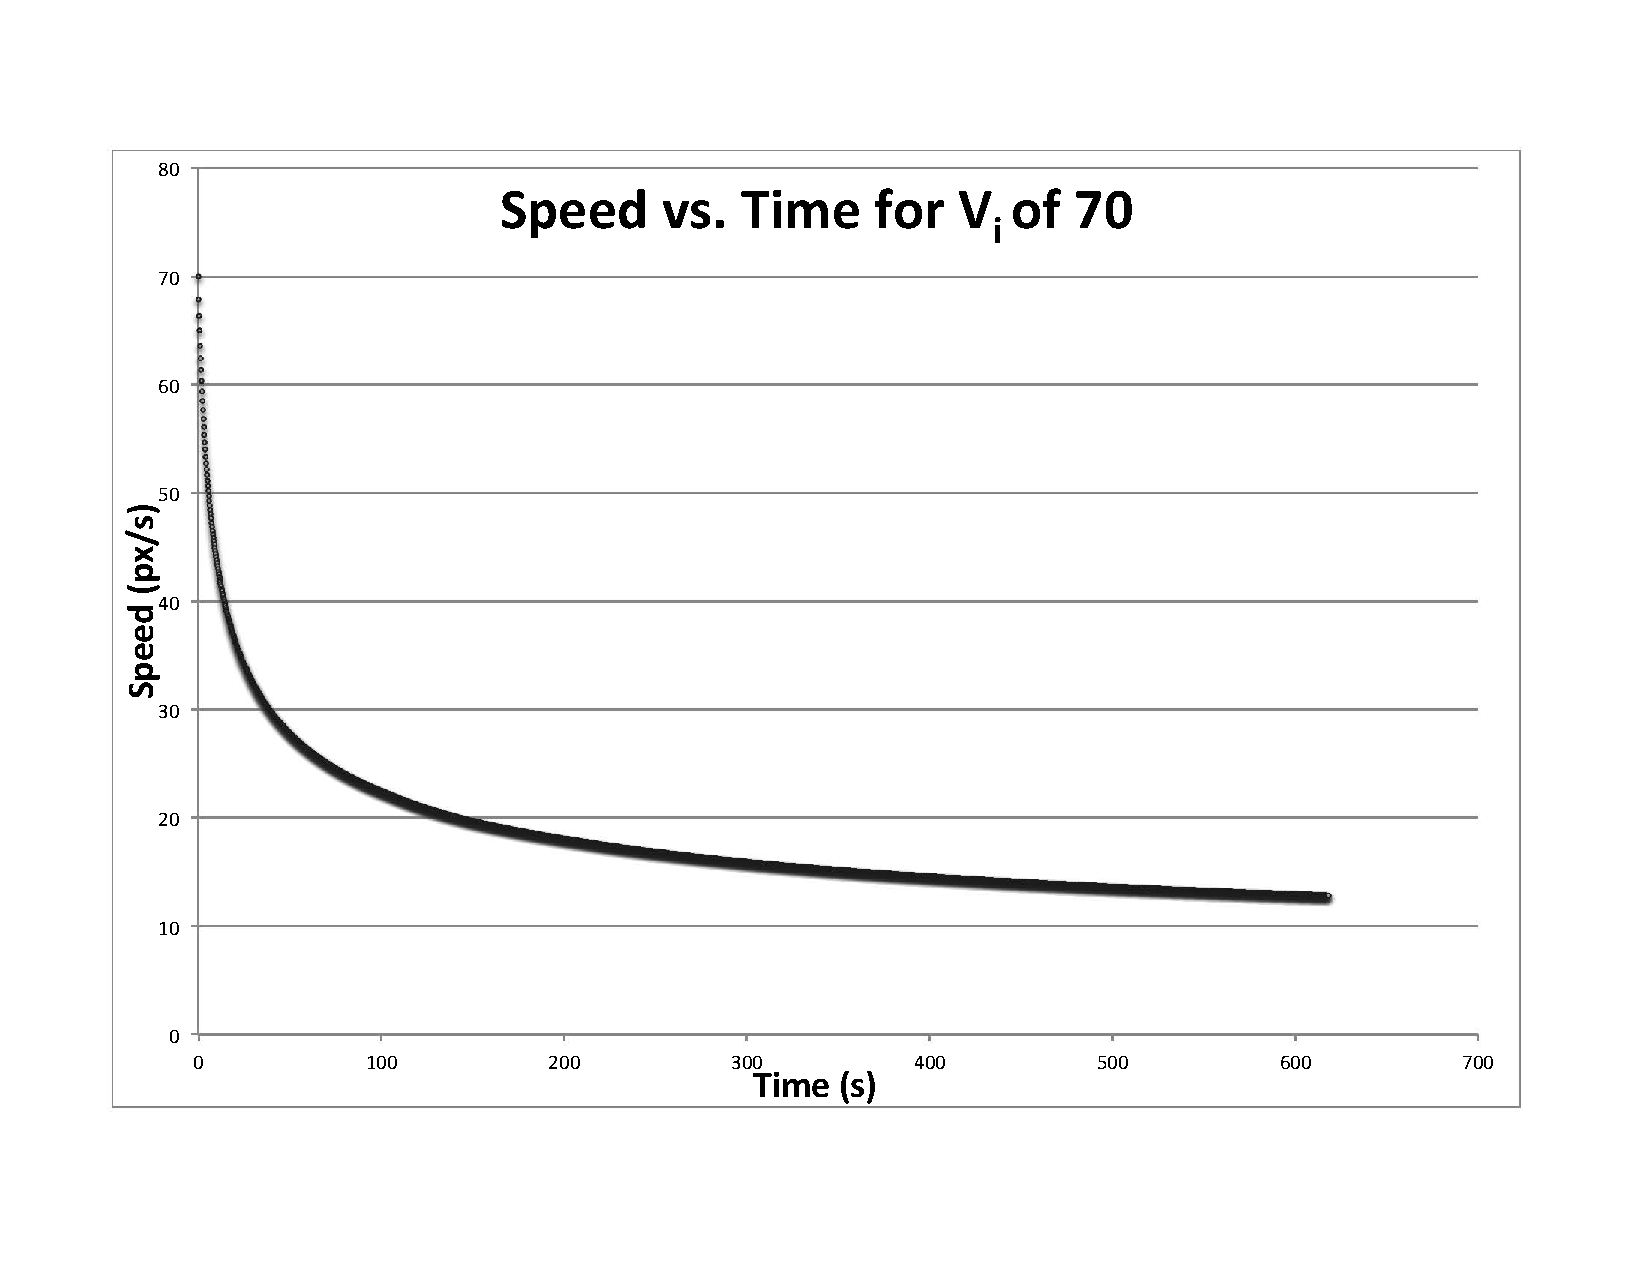
\includegraphics[width=9.5cm]{fig3.pdf}

	\label{fig:data1}
\end{figure}
\end{frame}


\subsection{Simulation \#6}

\begin{frame}

\frametitle{Simulation \#6: Kepler's 2nd law}

\begin{itemize}

\item Early 1600's Johannes Kepler proposed laws explaining how planets orbit the sun

 \item Law \#2:``The radius vector drawn from the Sun to a planet sweeps out equal areas in equal time intervals''

\item Simulation shows constant $\frac{dA}{dt}$

\end{itemize}
\end{frame}






\begin{frame}
\frametitle{Derivation of Kepler's 2nd Law}

\begin{itemize}

\item Gravity force is \textit{central} force

\item $
\vec{\tau} = \vec{r}\times\vec{F_g} = \frac{d\vec{L}}{dt}
$

\item $
 \vec{L} = \vec{r}\times \vec{p} = M_p \vec{r}\times\vec{v} 
 $

\item $
L = M_p \left|\vec{r} \times \vec{v}\right|
$

\begin{figure}[h] 
	\centering
		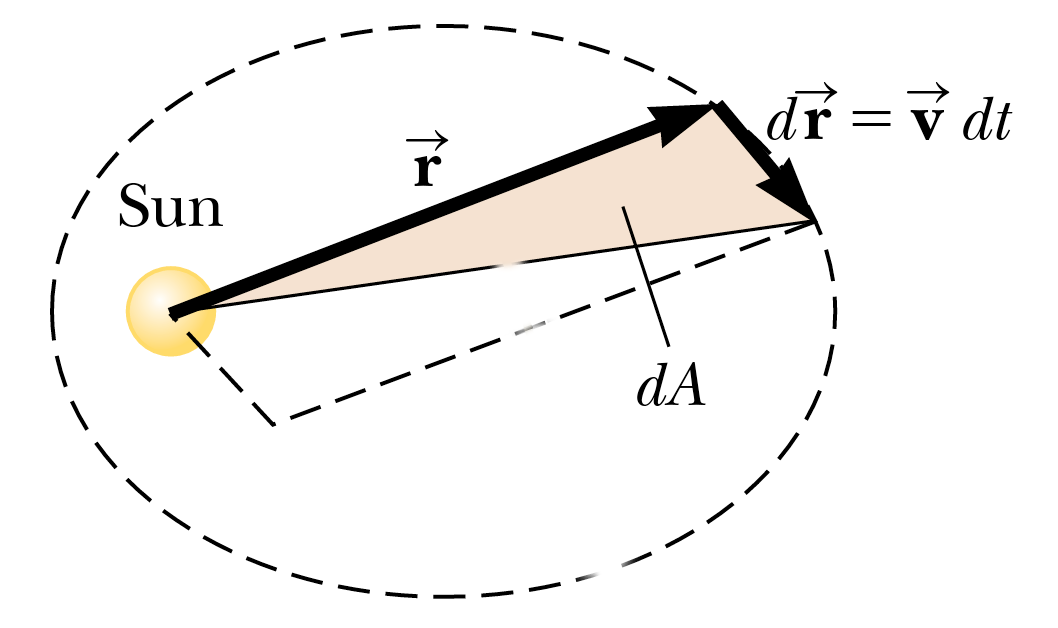
\includegraphics[width=5cm]{sun2.png}
	\caption{Relationship between  $\vec{r}$ and $d\vec{r}$}
	\label{fig:sun2}
\end{figure}





\end{itemize}


\end{frame}


\begin{frame}
\frametitle{Derivation of Kepler's 2nd Law (Continued)}

\begin{itemize}

\item $|\vec{r} \times d\vec{r}|$  area of parallelogram


\item $ dA = \frac{1}{2}|\vec{r} \times d\vec{r}| = \frac{1}{2}\left|\vec{r} \times \vec{v} dt \right| = \frac{1}{2}\left|\vec{r} \times \vec{v}\right| dt  $

\item From before, $\left|\vec{r} \times \vec{v}\right| = \frac{L}{M_p} $

\item $ dA = \frac{1}{2}\left(\frac{L}{M_p}\right)dt  $



\vspace{1cm}
\item $
\frac{dA}{dt} = \frac{1}{2}\left(\frac{L}{M_p}\right)
$

\item $L$ and $M_p$ are constants

\end{itemize}


\end{frame}

\begin{frame}
\frametitle{Kepler's 2nd Law}

\begin{figure}[h] 
	\centering
		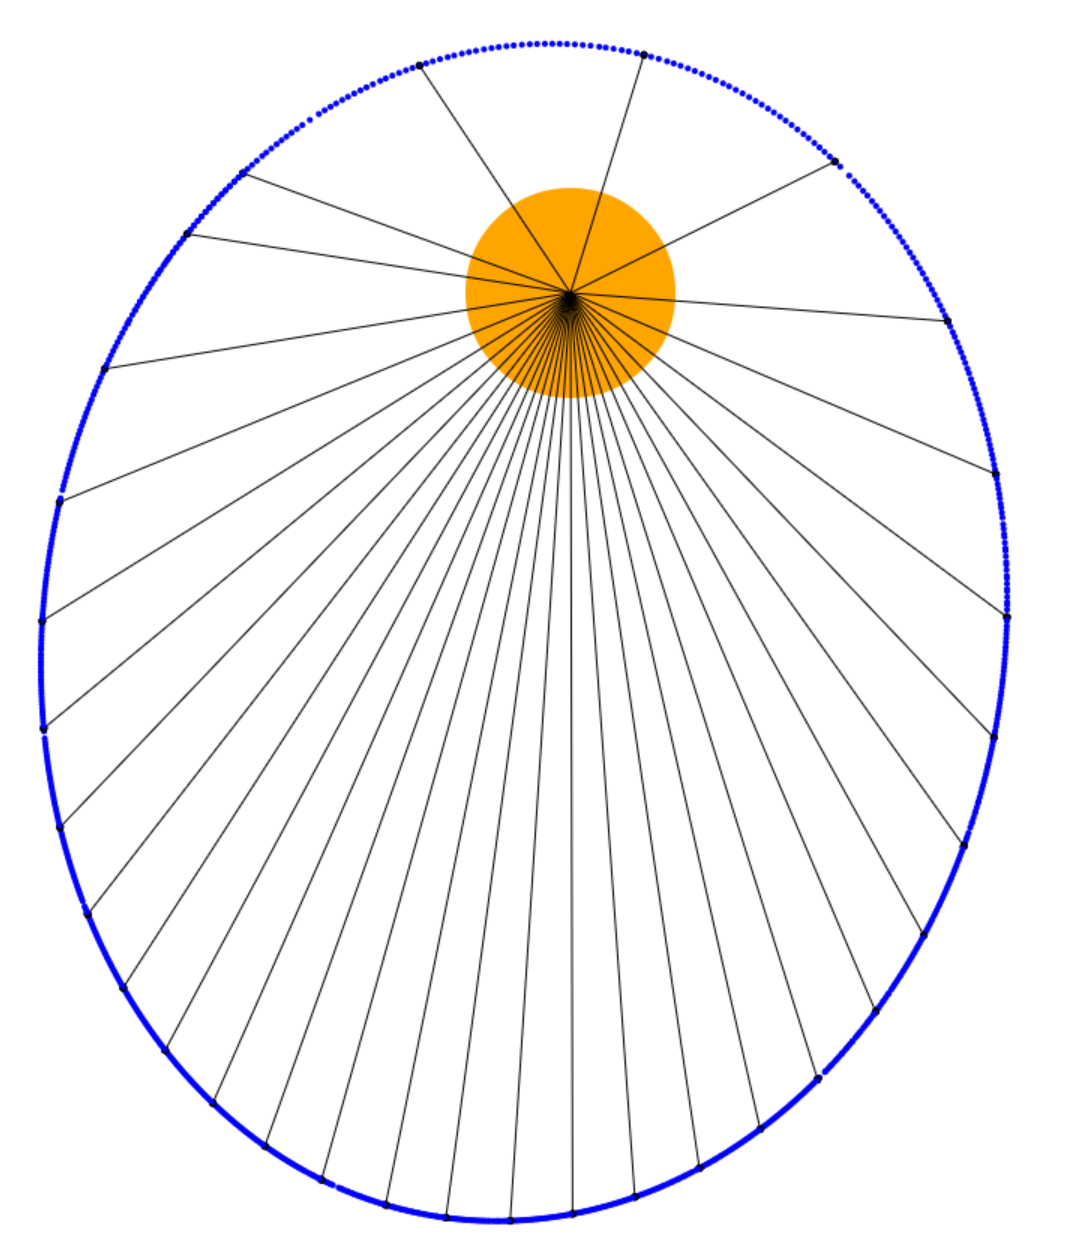
\includegraphics[width=5cm]{keplerscreenshot.png}

			\caption{Screenshot of Kepler Law test simulation}


	\label{fig:rigidbody}
\end{figure}

\end{frame}


\section{Chapter 3}
\subsection{Simulation \#3}

\begin{frame}

\frametitle{Chapter 3: Rotational Motion}

\begin{itemize}

\item $
\vec{\tau} = \vec{r} \times \vec{F}
$

\item $
I =   \int  r^2 dm
$








\begin{figure}[h] 
	\centering
		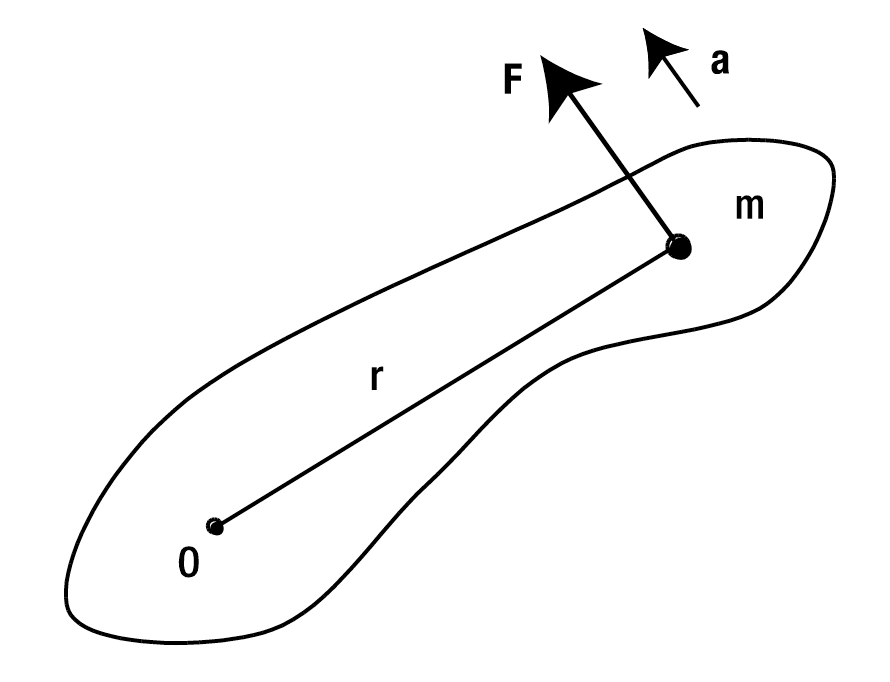
\includegraphics[width=4cm]{rigidbody.png}

	\label{fig:rigidbody}
\end{figure}

\end{itemize}

\end{frame}





\begin{frame}
\frametitle{Chapter 3: Rotational Motion}

\begin{itemize}

\item Newton's 2nd law for rotation

\item $
\vec{T} = I \vec{\alpha}
$


\vspace{1cm}

\item Program updates $\omega$ by calculating $\alpha$ from $T$ and $I$.
\end{itemize}
\end{frame}




\section{Conclusion}

\begin{frame}
\frametitle{Conclusion}

\begin{itemize}

\item Simulations can be made very accurate with JavaScript

\item Advantages of simulations involve sending instructions

\item Future improvements could involve 3D

\end{itemize}

\end{frame}
















































%------------------------------------------------



%------------------------------------------------




%\begin{frame}
%\frametitle{Multiple Columns}
%\begin{columns}[c] % The "c" option specifies centered vertical alignment while the "t" option is used for top vertical alignment
%
%\column{.45\textwidth} % Left column and width
%\textbf{Heading}
%\begin{enumerate}
%\item Statement
%\item Explanation
%\item Example
%\end{enumerate}
%
%\column{.5\textwidth} % Right column and width
%Lorem ipsum dolor sit amet, consectetur adipiscing elit. Integer lectus nisl, ultricies in feugiat rutrum, porttitor sit amet augue. Aliquam ut tortor mauris. Sed volutpat ante purus, quis accumsan dolor.
%
%\end{columns}
%\end{frame}
%
%%------------------------------------------------
%\section{Second Section}
%------------------------------------------------

%\begin{frame}
%\frametitle{Table}
%\begin{table}
%\begin{tabular}{l l l}
%\toprule
%\textbf{Treatments} & \textbf{Response 1} & \textbf{Response 2}\\
%\midrule
%Treatment 1 & 0.0003262 & 0.562 \\
%Treatment 2 & 0.0015681 & 0.910 \\
%Treatment 3 & 0.0009271 & 0.296 \\
%\bottomrule
%\end{tabular}
%\caption{Table caption}
%\end{table}
%\end{frame}
%
%------------------------------------------------
%
%\begin{frame}
%\frametitle{Theorem}
%\begin{theorem}[Mass--energy equivalence]
%$E = mc^2$
%\end{theorem}
%\end{frame}
%
%------------------------------------------------
%
%\begin{frame}[fragile] % Need to use the fragile option when verbatim is used in the slide
%\frametitle{Verbatim}
%\begin{example}[Theorem Slide Code]
%\begin{verbatim}
%\begin{frame}
%\frametitle{Theorem}
%\begin{theorem}[Mass--energy equivalence]
%$E = mc^2$
%\end{theorem}
%\end{frame}\end{verbatim}
%\end{example}
%\end{frame}
%
%------------------------------------------------
%
%\begin{frame}
%\frametitle{Figure}
%Uncomment the code on this slide to include your own image from the same directory as the template .TeX file.
%\begin{figure}
%\includegraphics[width=0.8\linewidth]{test}
%\end{figure}
%\end{frame}
%
%------------------------------------------------
%
%\begin{frame}[fragile] % Need to use the fragile option when verbatim is used in the slide
%\frametitle{Citation}
%An example of the \verb|\cite| command to cite within the presentation:\\~
%
%This statement requires citation \cite{p1}.
%\end{frame}
%
%------------------------------------------------

%\begin{frame}
%\frametitle{References}
%\footnotesize{
%\begin{thebibliography}{99} % Beamer does not support BibTeX so references must be inserted manually as below
%\bibitem[Smith, 2012]{p1} John Smith (2012)
%\newblock Title of the publication
%\newblock \emph{Journal Name} 12(3), 45 -- 678.
%\end{thebibliography}
%}
%\end{frame}
%
%------------------------------------------------

\begin{frame}
\Huge{\centerline{Thank You}}
\end{frame}

%----------------------------------------------------------------------------------------

\end{document} 